\documentclass{beamer}

\usepackage{framed}
\usepackage{graphicx}
\usepackage{listings}
\usepackage{hyperref}

\begin{document}

\title[Review and Struct Functions]{A Brief Review and Struct Functions}
\author[Z. Latta]{Zach Latta}
\date[December 2013]{December 04, 2013}

\frame{\titlepage}

\begin{frame}[fragile]
  \frametitle{For Loop}
  \begin{itemize}
    \item Lets you repeat code.
  \end{itemize}

  \begin{lstlisting}[language=go]
  for i := 1; i <= 3; i++ {
    fmt.Println(i)
  }
  \end{lstlisting}

  Expected output:
  \begin{lstlisting}[language=go]
  1
  2
  3
  \end{lstlisting}
\end{frame}

\begin{frame}[fragile]
  \frametitle{For Loop Exercise}
  Write a program that prints ``Hi'' 100 times.

  Expected output:
  \begin{lstlisting}[language=go]
  Hi
  Hi
  Hi
  ...
  \end{lstlisting}

  When you're done, submit to \url{http://pilot.eshsrobotics.com}
\end{frame}

\begin{frame}[fragile]
  \frametitle{Functions}
  \begin{itemize}
    \item Let you reuse code.
  \end{itemize}

  \begin{lstlisting}[language=go]
  func main() {
    log("Program started.")

    n := 42 + 5
    log("Addition completed succesfully.")

    log("Program finished.")
  }

  func log(msg string) {
    fmt.Println("LOG:", msg)
  }
  \end{lstlisting}
\end{frame}

\begin{frame}[fragile]
  \frametitle{Functions Exercise}
  Write a function that takes two ints, adds them together, and prints the
  result. Demonstrate its usage in your main function.

  \begin{lstlisting}[language=go]
  yourFunction(10, 5)
  >> 15
  yourFuncion(42, 13)
  >> 55
  \end{lstlisting}

  Make sure you give your function a descriptive name! Submit your completed
  program to \url{http://pilot.eshsrobotics.com}.
\end{frame}

\begin{frame}
  \frametitle{Remember Doge?}
  
\includegraphics[height=3.0in]{doge}
\end{frame}

\begin{frame}
  
\includegraphics[height=3.0in]{compsci_doge}
\end{frame}

\begin{frame}
  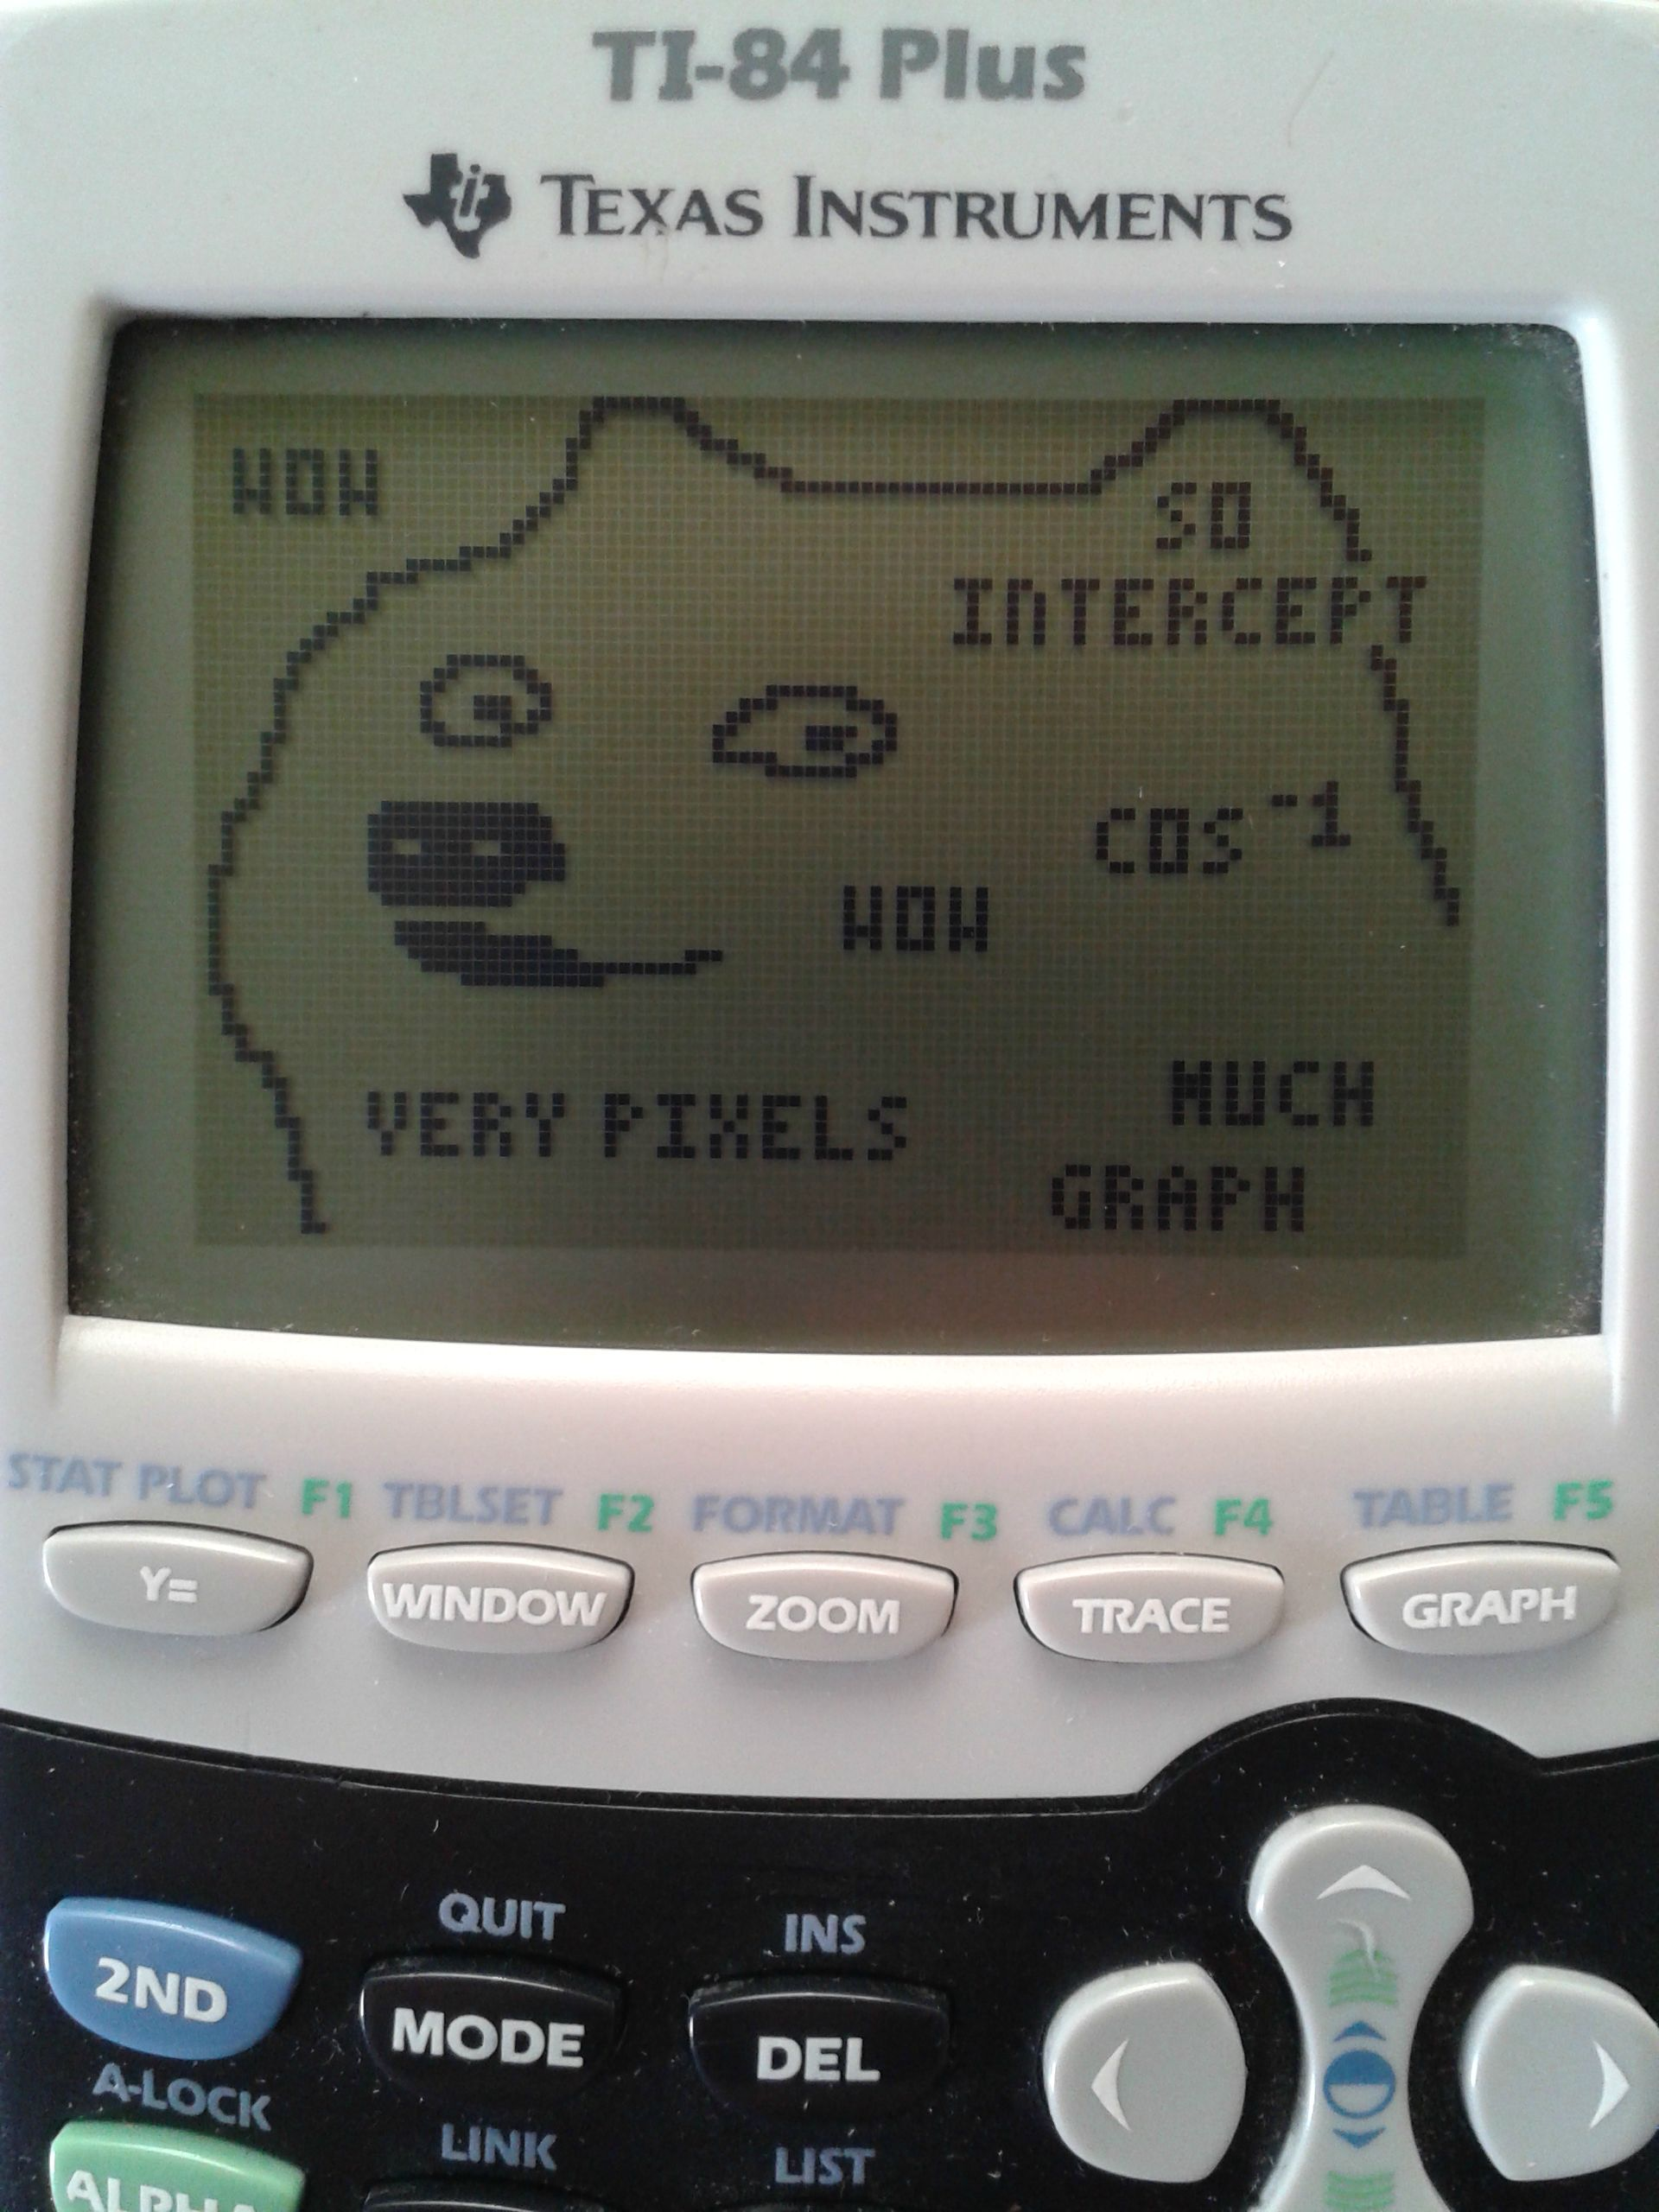
\includegraphics[height=3.0in]{calc_doge}
\end{frame}

\begin{frame}
  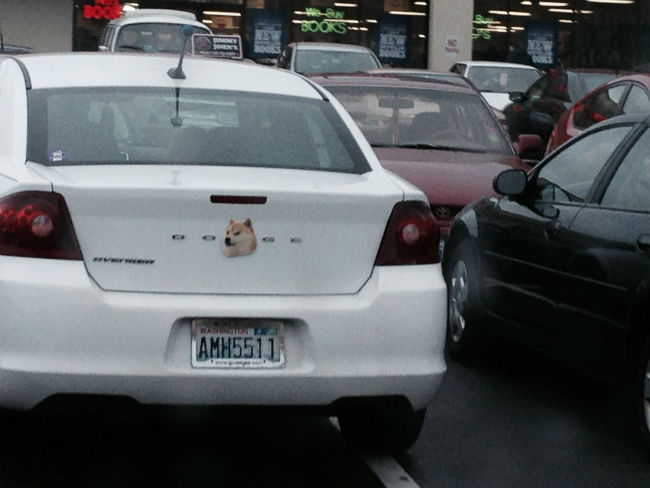
\includegraphics[height=3.0in]{dodge_doge}
\end{frame}

\begin{frame}[fragile]
  \frametitle{Doge and Structs}

  \begin{lstlisting}[language=go]
  type Doge struct {
    Name string
    Phrases []string
  }

  func main() {
    doge := Doge{
      Name: "John",
      Phrases: []string{"Such wow", "Many word"},
    }
    fmt.Println(doge.Name)

    for i := 0; i < len(doge.Phrases); i++ {
      fmt.Println(doge.Phrases[i])
    }
  }
  \end{lstlisting}
\end{frame}

\begin{frame}[fragile]
  \frametitle{Struct Functions}

  \begin{lstlisting}[language=go]
  type Doge struct {
    Name    string
    Phrases []string
  }

  func (d *Doge) PrintPhrases() {
    for i := 0; i < len(d.Phrases); i++ {
      fmt.Println(d.Phrases[0])
    }
  }

  func main() {
    doge := Doge{
      Name: "John",
      Phrases: []string{"Such wow", "Many cold"},
    }
    doge.PrintPhrases()
  }
  \end{lstlisting}
\end{frame}

\begin{frame}[fragile]
  \frametitle{Struct Functions Exercise}

  \begin{itemize}
    \item Write your own doge struct with functions.
    \item Struct Fields
      \begin{itemize}
        \item Name - Doge's name
        \item Phrases - All of the doge's available phrases
        \item Lost - Whether or not the doge is lost
      \end{itemize}
    \item Struct Functions
      \begin{itemize}
        \item Print phrases - Prints each of the doge's phrases
        \item Random phrase - Prints a random phrase
        \item Found - Makes the doge no longer lost
      \end{itemize}
  \end{itemize}

  Code from the last slide is available at
  \url{http://pilot.eshsrobotics.com/view/3}. Submit your finished code to
  \url{http://pilot.eshsrobotics.com}.
\end{frame}

\end{document}
